x\section{Audio System}
\label{dmx_section}
Like every other I/O in the engine, the audio system was abstracted behind an interface. To fulfit \doom's Core expectations such a system had to implement not less than twenty functions covering SFX, Music, and also Timer.\\
\par
 \begin{figure}[H]
\centering  
\begin{tabularx}{\textwidth}{ L{0.6}  L{1.4}}
  \toprule
  \textbf{Method} &  \textbf{Usage}\\

  \toprule 
  I\_StartupSound & Initialize Audio system, detect audio hardware\\
  I\_SetChannels & Set number of channels and sample rate\\
  \toprule 
   
I\_RegisterSong & \\
I\_SetMusicVolume &\\
I\_PlaySong &\\
I\_PauseSong &\\
I\_ResumeSong &\\
I\_StopSong &\\
I\_UnRegisterSong & \\




  \toprule 
I\_GetSfxLumpNum & Load audio sample from WAD and associate it with an id.\\
I\_StartSound & Start playing SFX sample\\
I\_StopSound & Stop playing SFX sample\\
I\_SoundIsPlaying & Test is SFX is playing\\
I\_UpdateSoundParams & Set pitch, left/right position and volume\\

  \toprule 
  
I\_StartupTimer &\\
I\_ShutdownTimer &\\

   \toprule
\end{tabularx}
\caption{\doom audio system interface}
\end{figure}



On NextStep this system was never a problem since only the timer function had to be implemented. On the PC side however the game engine had to have sound effects and musics. The difficulty of the task was the fragmentation of the sound card market which had increased exponentially since Wolfesnstein 3D. The previous title required tremendous effort to support four sound sources. Two years later there were more than fifteen chips available, all with different types of bugs, kirks and technologies.\\
\par
To make things worse, the departure of Jason Blochowiak  at left id Software with both a shortage of expertise and enthousiasm toward audio. They solved the problem by throwing money at it and licensed DMX library. For the price of its license, the library authored by Paul J. Radek offered an all-in-one audio solution. With support for all major sound cards, convenient means to detect them, support of many sound and music formats, and an easy way to integrate with any game engine, DMX was a perfect fit which undoubtedly saved id several months of development.\\
\par
The abstraction layer provided by DMX was a colossal task. The comment before the function in charge of detecting the hardware leaves no ambiguity regarding how big an issue it was to tackle.\\
\par
\ccode{whypcssucks.c}
\par
With DMX backing the sound system, ten audio chipsets were supported.\\
\par
\ccode{cardenum_t.c}
\par
Running on an operating system supporting neither threads nor processes, there was seemingly not way to generate both the video and the audio output simultaneously.\\
\par
 An attentive reader will have noticed the hardware section mentioning the PC two chipsets i8259 (Programmable Interrupt Controller: PIC) and i8254 a (Programmable Interval Timers: TIC). Together they can be setup to stop (a.k.a interrupt :P) the engine execution and call into DMX routine\footnote{The way PIC and TIC interact is extensively detailed in "Game Engine Black Book: Wolfesntein 3D".}.\\
\par
Upon initialization, DMX installs itself as a TSR via the PIC and the TIC to be called at 140Hz. Upon awakening the TSR took care of feeding the audio device with music and sound effect data which had been provided by the engine. Since the were no other source of time on the machine, DMX was also in charge of generating the heartbeat via a variable counter called \cw{ticcount}.
\par


\scaleddrawing{1}{sound_manager_architecture}{DMX architecture}
With such an architecture there are actually two systems but the TSR has additional constraints. The engine makes sure the audio data is in RAM and instruct DMX of what to play. When an interrupt is triggered, DMX has only a few milliseconds to refill the sound card buffers and go back to sleep.\\
\par
 This is why audio allocation get a special treatment in the zone allocator. The audio system simply has no time to recover from a memory miss (nor could it since it has no access to the wad or memory allocator. Audio data had to be ready at all time it could be used.
\pagebreak

\subsubsection{Audio Data: Formats and Lumps}
The wad archive contains hundreds of lumps containing five type of audio data.
\begin{itemize}
  \item PC Speaker Sound Effects
  \item Soundcard Sound Effects
  \item Music
  \item GENMIDI
  \item DMXGUS
\end{itemize}
\par
PC Speaker audio was meant for PC equipped with no sound card. The PC Speaker was actually a beeper capable of only square waves and meant to emit boot up diagnostic noise. There were ways to make it generate something less irritating by changing the square frequency every 1/140th of a second. This is exactly the format \doom is using with a stream of byte dictating frequencies. These samples are stored in lumps starting with \cw{DP}.\\
\par
 Digitized audio sample are recorded as 8-bit, 11025 Hz, mono PCM stream without even a header. It is a format DMX can use directly without transformation.  These samples are stored in lumps starting with \cw{DS}.\\
\par
Music are stored in Genera MIDI format. With eight channels for instruments and a ninth for the drums. Channels were limited to 9 by early Sound Blaster cards. These samples are stored in lumps starting with \cw{D\_}.\\
\par
GENMIDI, TODO: Dig inside article "The dark and forgotten art of GENMIDI".\\\\
\par
DMXGUS\\
\par
\pagebreak



Dealing with so much complexity proved difficult for DMX. Some of the craziness Paul Radek had to deal with surfaced in a post on \cw{vogons.org}\footnote{Forum thread: "Gravis Ultrasound - Hardware Mixing Game List".}.\\





\fq{All of the sound effects are now mixed in software, rather than on the GUS hardware. Why, you ask? Because of several reasons. First, is that the GF1 chip has a minimal ramp time that is much to long for very sharp effects. Second, because loading of the MUSIC patches uses all of the GUS memory, I had to DMA all eight sound effects to the card when played. This intern exposed a bug in the GF1 chip that Gravis did not find until my code started to beat on it. The bug would cause the bus to freeze and any program with it. The workaround is to keep DMA activities to a minimum by mixing in software and transfering only 1 channel to the GUS. But since the GF1 can't support auto-initialize DMA, and because the only way to play interleaved data on the card is to set two voices pointing into a single patch and setting the frequency so the every other sample is skipped, you don't get the benifit of sample smoothing from the GF1.\\
\par
Sorry, but that's the way it has to be :(\\
}
{Paul Radek, Digital Expressions, Inc.}\\
\par

The library evolved during the development of \doom and sometimesAPI changes introduced bugs. Gravis UltraSound was broken with v1.666. Support for Audio Spectrum was also broken but it was not too bad since the card had an option to emulate sound blasters\footnote{Source: John Romero post on \cw{alt.games.doom}.}.\\
\par
The problem was partly due to poor API practices on Digital Expressions side and probably hasty support on id Software part. \doom did ship with a significant bug. The engine was originally supposed to emit sounds at random pitch to avoid monotony for which it used DMX function \cw{SFX\_PlayPatch}.\\
\par
\ccode{dmx_before.c}





However the DMX API was latter modified in an interesting way. It may not be immediately apparent but function \cw{SFX\_PlayPatch} parameters have been reversed.\\
\par
\ccode{dmx_after.c}\\
\par
 The game shipped without the random pitch feature, instead randomly balancing sound between the left and right channel.\\
\par
\ccode{I_StartSound.c}\\
\par
In retrospect John Carmack regretted using DMX because it led to issues when open sourcing the game engine (it is unknown if Paul Radek was unwilling to open source DMX or if id software was unwilling to negotiate with him).\\
\par
\fq{
Our biggest mistake during DOOM development was the contracting of an  
outside party to do dos sound drivers.  Because we had this black box  
functionality coming, I didn't simulate it under NS.  BAAAAAD mistake.   
All future work will be entirely developed under NS, with only DMA  
buffer flipping being the hardware layer.  We will probably also run  
midi under NS for music (which will be dynamically tuned to the game  
situation in Quake).}{John Carmack}\\
\par
Judging by usenet message posted by John Romero, it sounds like relationship between Radek and id software were tense with bad names being thrown\footnote{Source: John Romero post on \cw{alt.games.doom}.}.\\
% \par
% \fq{Hey, everybody!  Thanks a lot for downloading DOOM II -- that's really "cool".   
% We love it when we send evaluation copies to magazine editors and some piece of  
% shit uploads the thing.  The DOOM II out there is the master copy we sent to GT  
% Interactive, our distributor.  If your GUS sound doesn't work, it's probably  
% because your IRQ is > 7.  Our sound code dork broke part of the sound support  
% while he was "expanding" it, so IRQs > 7 don't work, Pro Audio Spectrum owners  
% now have to run their SB-emulation driver (no more native support), etc.  The  
% sound guy is a real shithead.  All these fuckups are in v1.666 as well --  
% sorry.  We have NO time to wait and hope that sound-dork fixes these problems,  
% as he's demonstrated in the past year and a half that he's incompetent.}{John Romero (alt.games.doom)}



\section{Sound Propagation}
How well enemies react to sounds makes a huge difference about how smart A.I is perceived. id Software made sure sound propagation was accurate. When a shot is fired in a sector, a fill flood algorithm propagates the noise.\\
\par
\ccode{P_RecursiveSound.c}\\

\begin{wrapfigure}[10]{r}{0.48\textwidth}
\centering
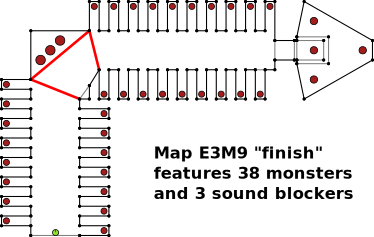
\includegraphics[width=.48\textwidth]{drawings/sound_blockers.pdf}
\end{wrapfigure}
  The sectors/portals format is leveraged, starting in the current player sector and flood-filling into adjacent sectors via portals (two-sided lines). Sound is stopped when either a door is encountered or when two "sound blockers" lines have been crossed. Map E3M9 features section with no less than 38 monsters. To lower A.I cost, three line blockers helped to maintain half of them dormant.\\
\par
Notice function \cw{P\_RecursiveSound} mention "waking up all monsters" but it never iterate over the list of things in the level. This is an interesting speed-up trick aimed at avoiding an expensive search to find all monsters to be awakened in each sector. Monsters always look up for the current sector's \cw{soundtarget} to pick a target. By simply assigning a value to \cw{sec->soundtarget}, all monsters in \cw{sec} automatically acquire the same target.\\
\par
\rawdrawing{E1M1_audio_sections}
\par
\subsubsection{Ambushing}
Map designers wanted to have sneaky monsters that could hide and wait to jump on a player. This is achieved via the MF\_AMBUSH that can be assigned to monsters. It doesn't make monsters deaf, it only makes them not seek the player until they make visual contact.


\subsubsection{Super Ambushing}
Sound propagation was used in a inventive way for map E1M9 super ambush.  The designers wanted the player to be ambushed after it had walked through the center of a pentagram.\\
\par
 As soon as it happened, monsters would start flooding the room, teleporting in the center of the "star". But without a scripting language available that was next to impossible to do since, as we will see in the A.I section, monsters can do only three things: Stay dormant, Pursue a target, and when they bump into walls and things, try a new direction.\\
\par
\begin{wrapfigure}[22]{r}{0.48\textwidth}
\centering
\includegraphics[width=.48\textwidth]{drawings/e1m9_sides.pdf}
\end{wrapfigure}

\par

To achieve the effect, they create an unaccessible "monster pool" room next to where they wanted the super ambush and filled it with monsters (red circles in the drawing). In the right bottom of the room, they place a teleporter, protected by walls.\\
\par
They created a very tiny pipe to allow sound to flow through so when the player was fighting in this room, all monsters in the "pool" room would have been awakened and tried to reach the player. Without a way to get there (the monsters at too big to go through the pipe and also the pipe is at ceiling level) monsters started to run in circle with a tendency to go toward the player location.\\
\par
The last piece of the super ambush was to have four lines around the center of the "star" which lowered the walls around the teleporter and place a bait on it (such a lots of health and ammunitions) to make sure the player would go there. The trap was set.\\
\par

As soon as the player walked on the trigger in the "star" room, the walls around the teleporter lowered, monsters moved toward it and "spawned". \\
\par
\trivia{Comments in the code suggest that monsters screaming awaken other monsters but it is not the case. It is unknonw why this feature was cut. Maybe it was too buggy or too expensive.}\\
\pagebreak

John Romero himself described how they placed the "pipes".\\
\par
\fq{We used sound zones in Wolfenstein 3D as another way to alert enemies to your presence. In DOOM, we did the same thing but used sectors as the conduits of audio travel. This was a really important part of making the game scary, as sound could leak all over the place and alert demons. You might see lots of little sector pipes that connect sectors together just to alert monsters-sectors that you'd never see because we put them way up high in the corner of a room. So, we paid a lot of attention to the sound flooding.}{John Romero, p29 in Scarydarkfast}\\
\par
The audio pipe in E1M9 super ambush is so well hidden in the ceiling that it is very hard to notice it with the vanilla engine. However opening the map with an editor such as Slade release the stratagem.\\
\par
\cfullimage{sound_conduit.png}{The audio conduit to awaken monsters and make them go to the teleporter is visible in the upper right corder.}